\section{Results}


\subsection{Hard Process Variables}

\begin{figure}[ht]
  \centering
  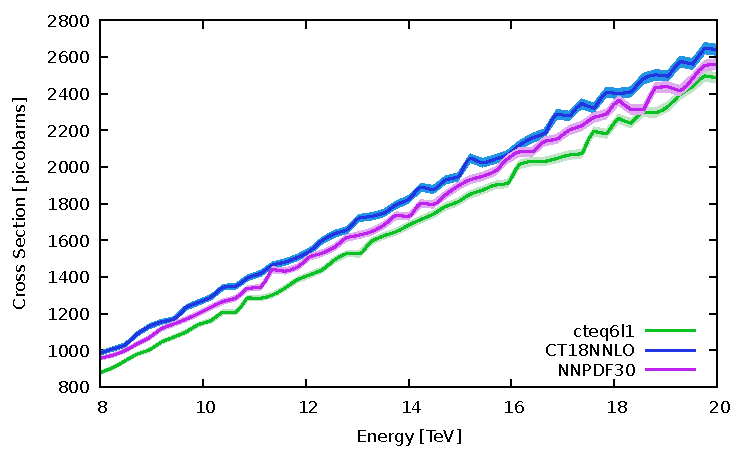
\includegraphics[width=0.7\textwidth]{./res/gfx/xs.pdf}
  \caption{Cross section dependence on center-of-mass energy for the three different candidate PDF sets.}
  \label{fig:ecm}
\end{figure}

Figure~\ref{fig:ecm} contains the curves depicting the dependence of the cross section on the center-of-mass energy of the main proton-proton collision, where the shaded region indicates the error. Importantly, for most other results we fix the number of iterations of the Monte Carlo iterations to be one million, but in this instance we drop it by a factor of 10 in order to increase speed. As we expect, the cross section grows monotonically with the ECM. Additionally, we can tell that the most accurate PDF sets increase the total value of the cross section due to the fact that they contain more corrections to the main process. Overall, the model performs well and as expected in this area.


\begin{figure}[ht]
  \centering
  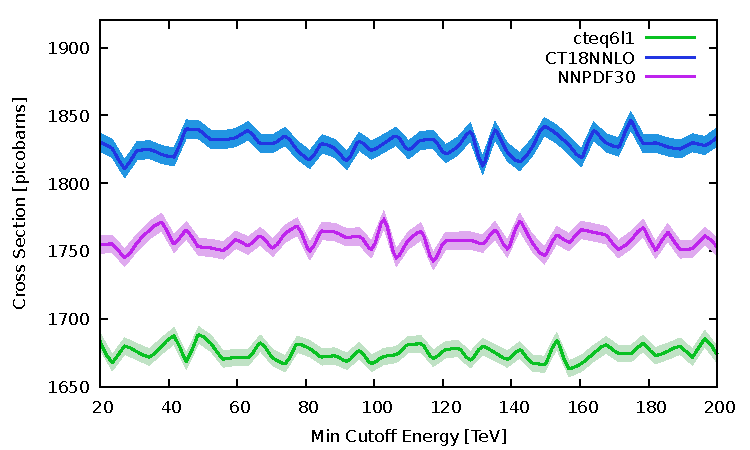
\includegraphics[width=0.45\textwidth]{./res/gfx/cutoff.pdf}
  %\includegraphics[width=0.45\textwidth]{./res/gfx/trans-energy.pdf} 
  \caption{Cross section dependence on the minimum cutoff energy (left) and transformed mass/width (right) for the three different candidate PDF sets.}
  \label{fig:cutoff-trans}
\end{figure}

Figure~\ref{fig:cutoff-trans} contains similar curves as Fig.~\ref{fig:ecm} but for the minimum cutoff energy and transformed mass/width. The $E_{\mathrm{CM}}$ was kept fixed at $\qty{14}{\tera\electronvolt}$. Interestingly, we still note that the more accurate PDF sets give larger results, but unexpectedly the two variables seem to have very little effect on the actual value of the cross section, though it does vary relatively widely. This is actually a very good thing, especially for the transformation mass/width, because that variable is an intermediate variable present only for calculational purposes, meaning that it \textit{shouldn't} have any effect on the cross section. Further, while the minimum cutoff energy technically has physical implications, we don't vary it low enough for those physical effects to manifest, meaning it also shouldn't have an effect.

We next show the dependence of the distributions for the events that were generated after varying the ECM. We know now that the changing of the intermediate calculation variables does not have a noticable effect on the cross section, which is the fundamental quantity influencing the generation of events via the hit-or-miss method. Therefore, we will not show their effect. Further, the energy of the output events is the only distribution which we will show, since it is has the most clear physical implications.

\begin{figure}[ht]
  \centering
  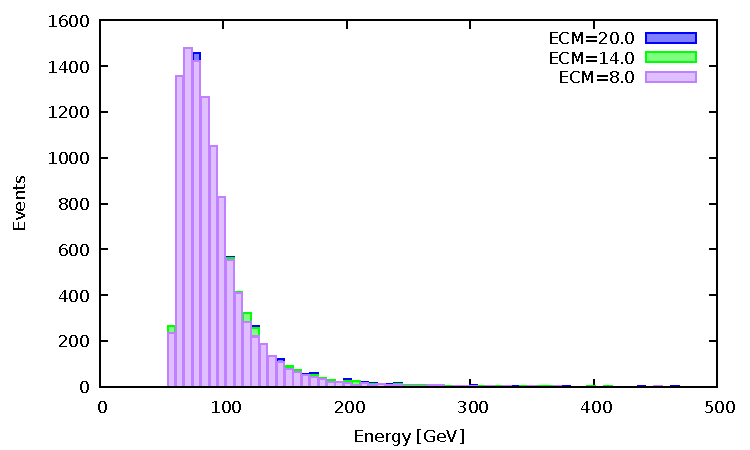
\includegraphics[width=0.7\textwidth]{./res/gfx/Q.pdf}
  \caption{$Q$ distributions after varying the center of mass energy.}
  \label{fig:q-dist}
\end{figure}

This is done in Figure~\ref{fig:q-dist}. It is surprisingly hard to notice, but the lower energy distribution has a sharper peak at a lower energy, while the higher energy distribution has a slightly more spread out peak but is noticeably shifted to the right. The extent to which it is shifted is much smaller than I would have expected, however, the fact that it is still obviously occurring means that the model is performing correctly. More work will be done, though, to look into whether it should be shifted as little as it is.

\subsection{Parton Showering}

Like mentioned previously, the parton showering process only spits out some distributions of the kinematics from the final state events, rather than any single numbers like the hard scattering part of the simulation. Also, similarly, some of these variables are intermediate calculation variables or have a less obviously physical significance, with the exception of the transverse momentum $p_T$.
\begin{figure}[ht]
  \centering
  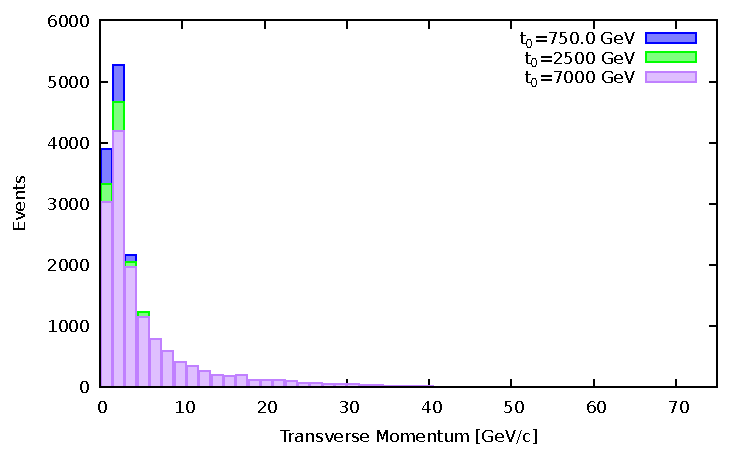
\includegraphics[width=0.45\textwidth]{./res/gfx/pt-fixed.pdf}
  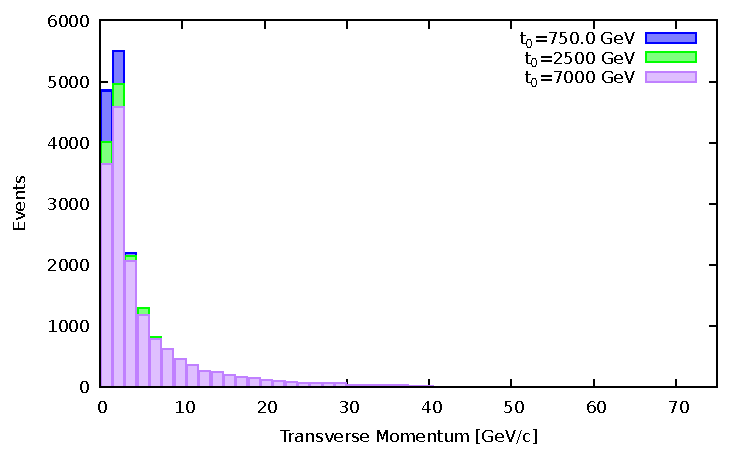
\includegraphics[width=0.45\textwidth]{./res/gfx/pt-variable.pdf}
  \caption{$p_T$ distributions for the generated parton showering events by varying the initial evolution energy for a fixed scale for the coupling (left) and a variable scale for the coupling (right).}
  \label{fig:pt-dist}
\end{figure}

Figure~\ref{pt-dist} contains two plots containing the output transverse momentum $p_T$ distributions for the generated parton showering events. On the left, the scale for the coupling $\alpha_s$ is kept fixed (and hence its value is also constant), and on the right, it is varied throughout each evolution.

The results here are a little bit more easy to see, and are as expected if we again consider the definition of the Sudakov factor. This factor determined the probability that the quark does \textit{not} emit a gluon from some initial scale $t_0$ to a final scale $t$. This means that for a particular evolution starting at a $t_0$ which higher compared to another at $t_0'$, it is essentially just as probable for the former evolution to emit a quark at a $t$ which is higher compared to the latter evolution at $t'$. The point is that it is more likely to emit gluons at a higher evolution scale when starting the evolution itself at a higher value (phrasing it this way makes it seem very intuitive, but it helps to have a mathematical grasp).

This is reflected in the plots since we see that the distributions corresponding to higher initial evolution scales are shifted to the right, corresponding to the fact that higher $p_T$ events are more likely. Evidently, the model is performing as expected in this regard. Another thing that we notice is that varying the coupling vs. keeping it fixed seems to have very little effect. This is expected: the fixed coupling is chosen to be at the scale of half of the initial evolution scale, meaning that, on average, it \textit{roughly} captures what the variable coupling would capture. Only super minor effects would matter, and those are impossible to tell in the graph. Further, the ``additional effects'' are only NLO effects, not NNLO or N$^3$LO (the order to which corrections to the couplings are known), meaning they are already very small.

\begin{figure}[ht]
  \centering
  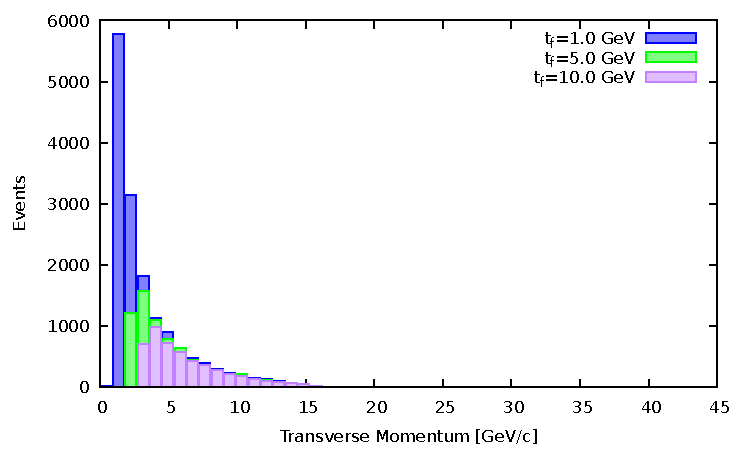
\includegraphics[width=0.45\textwidth]{./res/gfx/pt2-fixed.pdf}
  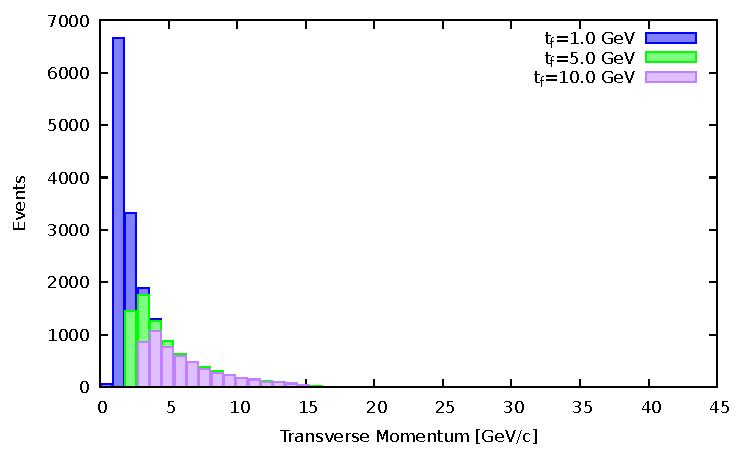
\includegraphics[width=0.45\textwidth]{./res/gfx/pt2-variable.pdf}
  \caption{$p_T$ distributions for the generated parton showering events by varying the evolution cutoff energy for a fixed scale for the coupling (left) and a variable scale for the coupling (right).}
  \label{fig:pt-dist2}
\end{figure}

In Figure~\ref{fig:pt-dist2}, I have done the same but this time by varying the final cutoff energy. This had the most notable effect of dramatically reducing the number of emissions that were generated by the end for the cases with higher cutoff. Further, the shape of each distribution is essentially identical, which makes sense. This is exactly as expected and shows further that the model works as expected.





%%% Local Variables:
%%% mode: LaTeX
%%% TeX-master: "../../Milestone6"
%%% End:
